\section{ROI-Based Fringe Tracking and Velocity Estimation}
\label{sec:roi_fringe_velocity}

In the experimental acquisition pipeline, frames of resolution $640 \times 480\text{ pixels}$ are captured at a sampling rate of $f_s = 30\text{ frames per second}$ (frame period $T_s = \frac{1}{f_s} \approx 33.33\text{ ms}$) \cref{sec:c270}. Rather than processing the entire sensor frame, a localized region of interest ($\text{ROI}$) spanning approximately one full fringe width is placed over a high-contrast region of the fringe pattern to track temporal irradiance modulation and fringe progression as movable mirror $M2$ translates along beam $(2)$ axis \cref{fig:schematic_michelson_interferometer}.



\subsection{ROI Mean-Irradiance Model}
\label{sec:roi_model_validity}

Starting from the two-beam interference model with fringe visibility of \cref{eq:visibility_irradiance} (\cref{sec:two_beam_interference}), the irradiance averaged over a small $\text{ROI}$ can be modeled as follows.

When spatially averaging $I(x, y, t_k)$ over a localized rectangular $\text{ROI}$ of dimensions $W \times H$ centered at $(x_0, y_0)$, the phase field can be approximated to first order as $\delta(x, y, t_k) \approx \delta_0(t_k) + k_x(x - x_0) + k_y(y - y_0)$, where $\delta_0(t_k)$ is the temporal phase at the $\text{ROI}$ center and $k_x = 2\pi/\Lambda_x$, $k_y = 2\pi/\Lambda_y$ represent the local spatial fringe wavenumbers. Assuming $I_0'$ and $V$ vary slowly across the small window, integrating over the $\text{ROI}$ yields:
\begin{equation}
    \bar{I}_{\text{ROI}}(t_k) \approx I_{\text{bg}} + I_{\text{amp}}\cos\!\bigl(\delta_0(t_k)\bigr)
    \label{eq:roi_irradiance_model_justified}
\end{equation}
where $I_{\text{bg}} \approx I_0'$ and the effective modulation amplitude is attenuated by spatial averaging according to
\begin{equation}
    I_{\text{amp}} \approx I_0'\,V\,\operatorname{sinc}\!\left(\frac{W}{\Lambda_x}\right)\operatorname{sinc}\!\left(\frac{H}{\Lambda_y}\right), \qquad \operatorname{sinc}(u) = \frac{\sin(\pi u)}{\pi u}
    \label{eq:roi_sinc_attenuation}
\end{equation}

\subsection{ROI Mean Irradiance and Classification}

\begin{figure}[htbp]
    \centering
    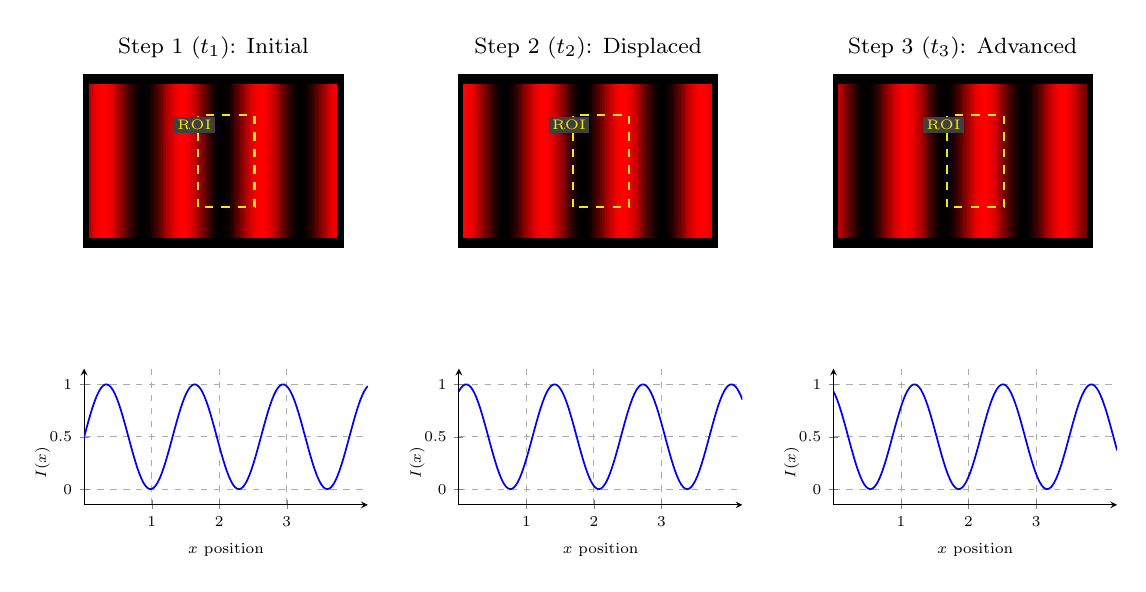
\begin{tikzpicture}[scale=0.78]
        % ==========================================
        % STEP 1: t_1 (Initial Position)
        % ==========================================
        \begin{scope}[shift={(0,0)}]
            % Camera View Box
            \draw[thick, fill=black] (0,4.2) rectangle (4.2,7.0);
            \node[above, font=\footnotesize] at (2.1,7.1) {Step 1 ($t_1$): Initial};
            \foreach \x in {0.10, 0.13, ..., 4.10} {
                \pgfmathsetmacro{\irradiance}{sin(\x * 280)*50 + 50}
                \draw[color=red!\irradiance!black, line width=0.45mm] (\x, 4.35) -- (\x, 6.85);
            }
            % ROI highlight box (~1 fringe wide: width = 1.35)
            \draw[dashed, yellow!95!black, thick] (1.85, 4.85) rectangle (2.77, 6.35);
            \node[fill=black!75, text=yellow!95!black, inner sep=1.2pt, font=\tiny, anchor=north west] at (1.45, 6.32) {ROI};
            \draw[thick] (0,4.2) rectangle (4.2,7.0);

            % Enlarged irradiance Plot
            \begin{axis}[
                at={(-0.4,0)},
                anchor=south west,
                width=6.2cm,
                height=3.8cm,
                xmin=0, xmax=4.2,
                ymin=-0.15, ymax=1.15,
                axis lines=left,
                xlabel={$x$ position},
                ylabel={$I(x)$},
                font=\scriptsize,
                xtick={1, 2, 3},
                ytick={0, 0.5, 1},
                grid=major,
                grid style={dashed, gray!65},
                xlabel style={below=1pt},
                ylabel style={left=1pt}
            ]
                \addplot[domain=0:4.2, samples=140, thick, blue] {sin(deg(x*4.8))*0.5 + 0.5};
            \end{axis}
        \end{scope}

        % ==========================================
        % STEP 2: t_2 (Intermediate Displacement)
        % ==========================================
        \begin{scope}[shift={(6.1,0)}]
            % Camera View Box
            \draw[thick, fill=black] (0,4.2) rectangle (4.2,7.0);
            \node[above, font=\footnotesize] at (2.1,7.1) {Step 2 ($t_2$): Displaced};
            \foreach \x in {0.10, 0.13, ..., 4.10} {
                \pgfmathsetmacro{\irradiance}{sin(\x * 280 + 60)*50 + 50}
                \draw[color=red!\irradiance!black, line width=0.45mm] (\x, 4.35) -- (\x, 6.85);
            }
            % ROI highlight box (~1 fringe wide: width = 1.35)
            \draw[dashed, yellow!95!black, thick] (1.85, 4.85) rectangle (2.77, 6.35);
            \node[fill=black!75, text=yellow!95!black, inner sep=1.2pt, font=\tiny, anchor=north west] at (1.45, 6.32) {ROI};
            \draw[thick] (0,4.2) rectangle (4.2,7.0);

            % Enlarged irradiance Plot
            \begin{axis}[
                at={(-0.4,0)},
                anchor=south west,
                width=6.2cm,
                height=3.8cm,
                xmin=0, xmax=4.2,
                ymin=-0.15, ymax=1.15,
                axis lines=left,
                xlabel={$x$ position},
                ylabel={$I(x)$},
                font=\scriptsize,
                xtick={1, 2, 3},
                ytick={0, 0.5, 1},
                grid=major,
                grid style={dashed, gray!65},
                xlabel style={below=1pt},
                ylabel style={left=1pt}
            ]
                \addplot[domain=0:4.2, samples=140, thick, blue] {sin(deg(x*4.8) + 60)*0.5 + 0.5};
            \end{axis}
        \end{scope}

        % ==========================================
        % STEP 3: t_3 (Advanced Displacement)
        % ==========================================
        \begin{scope}[shift={(12.2,0)}]
            % Camera View Box
            \draw[thick, fill=black] (0,4.2) rectangle (4.2,7.0);
            \node[above, font=\footnotesize] at (2.1,7.1) {Step 3 ($t_3$): Advanced};
            \foreach \x in {0.10, 0.13, ..., 4.10} {
                \pgfmathsetmacro{\irradiance}{sin(\x * 280 + 120)*50 + 50}
                \draw[color=red!\irradiance!black, line width=0.45mm] (\x, 4.35) -- (\x, 6.85);
            }
            % ROI highlight box (~1 fringe wide: width = 1.35)
            \draw[dashed, yellow!95!black, thick] (1.85, 4.85) rectangle (2.77, 6.35);
            \node[fill=black!75, text=yellow!95!black, inner sep=1.2pt, font=\tiny, anchor=north west] at (1.45, 6.32) {ROI};
            \draw[thick] (0,4.2) rectangle (4.2,7.0);

            % Enlarged irradiance Plot
            \begin{axis}[
                at={(-0.4,0)},
                anchor=south west,
                width=6.2cm,
                height=3.8cm,
                xmin=0, xmax=4.2,
                ymin=-0.15, ymax=1.15,
                axis lines=left,
                xlabel={$x$ position},
                ylabel={$I(x)$},
                font=\scriptsize,
                xtick={1, 2, 3},
                ytick={0, 0.5, 1},
                grid=major,
                grid style={dashed, gray!65},
                xlabel style={below=1pt},
                ylabel style={left=1pt}
            ]
                \addplot[domain=0:4.2, samples=140, thick, blue] {sin(deg(x*4.8) + 120)*0.5 + 0.5};
            \end{axis}
        \end{scope}
    \end{tikzpicture}
    \caption{Sequential time-steps ($t_1, t_2, t_3$) showing the fringe field, a single-fringe-width $\text{ROI}$ window, and 1D irradiance profiles $I(x)$ as movable mirror $M2$ translates.}
    \label{fig:three_step_fringes}
\end{figure}


For discrete frame index $k = 0, 1, 2, \dots$ acquired at time $t_k = k T_s = \frac{k}{f_s}$, let $I(x, y, t_k)$ denote the pixel irradiance within the $\text{ROI}$ (comprising $N_{\text{ROI}}$ pixels). The spatial mean irradiance inside the $\text{ROI}$ at frame $k$ is
\begin{equation}
    \bar{I}_{\text{ROI}}(t_k) = \frac{1}{N_{\text{ROI}}} \sum_{(x, y) \in \text{ROI}} I(x, y, t_k)
    \label{eq:roi_mean_irradiance}
\end{equation}

Neglecting slow variations, $\bar{I}_{\text{ROI}}(t_k)$ oscillates quasi-periodically with the interference phase difference $\delta(t_k)$:
\begin{equation}
    \bar{I}_{\text{ROI}}(t_k) \approx I_{\text{bg}} + I_{\text{amp}} \cos\!\bigl(\delta(t_k)\bigr)
    \label{eq:roi_irradiance_model}
\end{equation}
where $I_{\text{bg}}$ is the mean background level and $I_{\text{amp}}$ is the effective fringe modulation amplitude within the $\text{ROI}$. Using running or window extrema $\bar{I}_{\max}$ and $\bar{I}_{\min}$ estimated from recent frames, the normalized ROI irradiance is
\begin{equation}
    \tilde{I}_{\text{ROI}}(t_k) = \frac{\bar{I}_{\text{ROI}}(t_k) - \bar{I}_{\min}}{\bar{I}_{\max} - \bar{I}_{\min}} \in [0, 1]
    \label{eq:normalized_roi_irradiance}
\end{equation}

Maxima (constructive fringe peaks passing across the $\text{ROI}$) and minima (destructive dark fringes passing across the $\text{ROI}$) are identified from $\bar{I}_{\text{ROI}}(t_k)$ and its discrete temporal difference $\Delta \bar{I}_k = \bar{I}_{\text{ROI}}(t_k) - \bar{I}_{\text{ROI}}(t_{k-1})$:
\begin{itemize}
    \item \textbf{Local Maximum (Bright Fringe Center in ROI):} $\bar{I}_{\text{ROI}}(t_k)$ reaches a peak (or $\tilde{I}_{\text{ROI}}(t_k) \to 1$) where $\Delta \bar{I}_k$ transitions from positive to non-positive, corresponding to $\delta = 2\pi m$
    \item \textbf{Local Minimum (Dark Fringe Center in ROI):} $\bar{I}_{\text{ROI}}(t_k)$ reaches a trough (or $\tilde{I}_{\text{ROI}}(t_k) \to 0$) where $\Delta \bar{I}_k$ transitions from negative to non-negative, corresponding to $\delta = (2m + 1) \pi$
\end{itemize}
Because a single irradiance value cannot distinguish the rising slope ($\frac{d\bar{I}}{dt} > 0$) from the falling slope ($\frac{d\bar{I}}{dt} < 0$) at intermediate brightness levels, inspecting prior frames $t_{k-1}, t_{k-2}, \dots$ is necessary to resolve phase evolution and determine direction of movement, an schematic of this behavior is shown in \cref{fig:three_step_fringes}.

\subsection{Determining Direction from Frame History}
By combining the temporal history of $\bar{I}_{\text{ROI}}$ with local spatial/feature displacement across consecutive frames:
\begin{enumerate}
    \item \textbf{Slope and Extremum Sequence:} Comparing $\bar{I}_{\text{ROI}}(t_k)$ against $\bar{I}_{\text{ROI}}(t_{k-1})$ and $\bar{I}_{\text{ROI}}(t_{k-2})$ establishes whether the $\text{ROI}$ is currently traversing a rising half-cycle or falling half-cycle between consecutive maxima and minima.
    \item \textbf{Spatial Fringe Progression Across Frames:} Tracking a local fringe feature (or cross-correlating a 1D irradiance profile across the $\text{ROI}$ between frames $t_{k-1}$ and $t_k$) yields the signed spatial shift $\Delta x_{\text{fringe}, k}$ along the local fringe normal.
\end{enumerate}
Let $s_k \in \{+1, -1\}$ denote the signed direction indicator determined from frame history.

\subsection{Displacement and Velocity Equations}
Each complete fringe cycle ($\Delta m = 1$, from one maximum to the next or one minimum to the next) corresponds to a round-trip optical path change of $\lambda$, which equals an axial displacement of mirror $M2$ given by
\begin{equation}
    \Delta d_{M2, k} = s_k\,\frac{\lambda}{2}\,\Delta m_k
    \label{eq:roi_step_displacement}
\end{equation}
where $\Delta m_k$ is the fractional or integer fringe count accumulated between frame $k-1$ and frame $k$ (for instance, $\Delta m_k = 0.5$ between an adjacent maximum and minimum).

Over the frame interval $T_s = 1/f_s$, the mean axial velocity of mirror $M2$ during step $k$ is
\begin{equation}
    v_{M2, k} = \frac{\Delta d_{M2, k}}{T_s} = s_k\,\frac{\lambda}{2}\,f_s\,\Delta m_k = s_k\,\frac{\lambda}{2}\,f_{\text{fringe}, k}
    \label{eq:roi_step_velocity}
\end{equation}
where $f_{\text{fringe}, k} = f_s\,\Delta m_k$ is the instantaneous fringe-crossing frequency in $\text{Hz}$ (fringes per second).


